\documentclass[11pt]{article}
% Preamble for Paper II (trimmed from the shared macros.tex of the source).
\usepackage[utf8]{inputenc}
\usepackage[T1]{fontenc}
\usepackage{lmodern}
\usepackage{amsmath,amssymb,amsthm,mathtools}
\usepackage[margin=1in]{geometry}
\usepackage[colorlinks=true,linkcolor=blue,citecolor=blue,urlcolor=blue]{hyperref}

% One numbering scheme, within sections (Theorem 2.1, Corollary 2.2, Lemma 3.1, ...).
\newtheorem{theorem}{Theorem}[section]
\newtheorem{corollary}[theorem]{Corollary}
\newtheorem{lemma}[theorem]{Lemma}
\newtheorem{proposition}[theorem]{Proposition}
\numberwithin{equation}{section}
\newtheorem*{thmH}{Theorem H}
\newtheorem*{thmJ}{Theorem J}

\newcommand{\R}{\mathbb{R}}
\newcommand{\Z}{\mathbb{Z}}
\newcommand{\E}{\mathbb{E}}
\renewcommand{\Pr}{\mathbb{P}}
\newcommand{\eps}{\varepsilon}
\newcommand{\ball}{B}
\newcommand{\Sph}{S}
\providecommand{\ip}[2]{\langle #1,#2\rangle}
\DeclareMathOperator{\dist}{dist}
\DeclareMathOperator{\vol}{vol}

% Notation of the proofs (formerly local to the source appendix).
\newcommand{\Cone}{\mathbf{1}}
\newcommand{\Cout}{\mathrm{out}}
\newcommand{\Cin}{\mathrm{in}}
\newcommand{\CB}{\mathcal{B}}
% Projection and affine hull.
\newcommand{\Cpr}{\operatorname{pr}}
\newcommand{\Caff}{\operatorname{aff}}


\title{The covering radius of flats spanned by random points in a convex body}
\author{Michael Werman\\[2pt]
\small School of Computer Science and Engineering, The Hebrew University of Jerusalem}
\date{}

\begin{document}
\maketitle

\begin{abstract}
Let $X_1,X_2,\dots$ be independent points in a convex body $\Omega\subset\R^d$ with a density $f$ that is continuous on $\Omega$, and
for $1\le j\le d-1$ let $\rho^{(n)}$ be the largest distance from a point of $\Omega$ to the nearest $j$-flat spanned by $j+1$ of
$X_1,\dots,X_n$. We prove that $n^{j+1}(\rho^{(n)})^{d-j}/\log n$ converges almost surely to $(j+1)!\,d(j+1)/((d-j)\min_\Omega h_f)$,
where $h_f(z)=\lim_{t\to0}t^{-(d-j)}\Pr(\dist(z,F)<t)$ for the flat $F$ through $j+1$ independent points with density $f$, and that
the points of $\Omega$ farthest from the spanned flats approach the set of minimizers of $h_f$. The proof combines Poissonization
with Harris's and Janson's inequalities on a discretization whose mesh tends to $0$, and, for $j\le d-2$, a restriction of the
spanned flats that controls the dependence through shared points. With the affine Blaschke--Petkantschin formula we compute the
limit for balls (for instance $54$ for planes and $10$ for lines in the unit $3$-ball) and for lines in a square.
\end{abstract}

\noindent\textbf{Keywords:} random flats, covering radius, coverage threshold, Janson's inequality, Blaschke--Petkantschin
formula, geometric probability.

\noindent\textbf{MSC2020:} 60D05 (primary); 52A22, 60C05, 60F15 (secondary).

\section{Introduction}

Take $n$ points in a convex body $\Omega\subset\R^d$. How far from all $j$-flats spanned by $j+1$ of them can a point of $\Omega$
be? For a finite set $P$ and a compact set $A$ let $\rho_A(P)$ be the largest distance from a point of $A$ to the nearest $j$-flat
through $j+1$ affinely independent points of $P$ ($+\infty$ if there is none), and $\rho^*_n=\inf\{\rho_\Omega(P):P\subset\Omega,\
|P|=n\}$. The $\rho$-neighbourhood of a $j$-flat meets $\Omega$ in a set of volume $O(\rho^{d-j})$, so covering $\Omega$ by
$\binom n{j+1}$ of them forces $\rho^*_n\ge c\,n^{-(j+1)/(d-j)}$ (for hyperplanes Bang's plank theorem \cite{Bang} gives the explicit
bound $\rho^*_n\ge w/(2\binom nd)$, $w$ the minimal width of $\Omega$). Conversely, $\rho^*_n=O(n^{-d})$ for hyperplanes in every convex
body \cite[Proposition~6.10]{Companion}, and $\rho^*_n=O(n^{-(j+1)/(d-j)})$ for $j$-flats in a ball \cite[Section~6.3]{Companion}.

Here the points are random: $X_1,X_2,\dots$ are independent with a density $f$ that is continuous on $\Omega$ (for instance
uniform), and $\rho^{(n)}_\Omega=\rho_\Omega(\{X_1,\dots,X_n\})$. Theorem~\ref{thm:main} shows that $n^{j+1}(\rho^{(n)}_\Omega)^{d-j}/\log n$
converges almost surely to an explicit constant, determined by the minimum of a profile $h_f$: the normalized probability that the
flat through $j+1$ independent points with density $f$ passes near a given point. So $\rho^{(n)}_\Omega/\rho^*_n=O((\log
n)^{1/(d-j)})$ almost surely, and by \cite{Companion} this is the true order for hyperplanes in every convex body and for $j$-flats
in a ball. The result is first order only; the fluctuations are open (Section~\ref{sec:remarks}).

Three ingredients may be of independent use. (i) Harris's and Janson's inequalities, applied to a discretization whose mesh tends
to $0$ for fixed $n$, give two-sided Poisson bounds for the probability that a point is uncovered and for pairs of points
(Lemmas~\ref{lem:poisson} and~\ref{lem:fam}). (ii) For $j\le d-2$ a sample point near $z$ lies on many flats near $z$; discarding
the $(j+1)$-sets with a $j$-subset spanning a flat very close to $z$ removes this dependence at negligible cost (Lemma~\ref{lem:share}).
(iii) By the affine Blaschke--Petkantschin formula \cite[Theorem~7.2.7]{SW}, $h_f(z)$ is an integral over the sections of $\Omega$ by
flats through $z$, which makes the constant computable (Corollary~\ref{cor:ball}, Section~\ref{sec:examples}).

\paragraph{Related work.} Theorem~\ref{thm:main} is a coverage threshold: $\rho^{(n)}_\Lambda<\eps$ if and only if the open
$\eps$-neighbourhoods of the spanned flats cover $\Lambda$. Janson \cite{Janson86} found the threshold and its Gumbel fluctuations
for coverage by independent small random sets; see \cite{Hall,Penrose,PH} for balls around random points and \cite{BCL} for caps
on the sphere. Our covering sets cross the whole body. Coverage by cylinders around independent random lines is studied in
\cite{DJY}, and for the Poisson line tessellation, whose lines are independent, extreme-value limits for the largest inradius are
known \cite{CH,Chenavier}. Here the $\binom n{j+1}$ flats are determined by $n$ points and are strongly dependent, yet at first order
the threshold is the one predicted by the Poisson clumping heuristic \cite{Aldous} for $\binom n{j+1}$ independent copies of the
flat. Random secants of a convex body \cite{Kingman,Coleman} and mean values for random simplices in a convex set \cite{Groemer} are
classical. For fixed $z$ the number of spanned flats near $z$ is a $U$-statistic; Poisson approximation for such counts and for
extremes of $U$-statistics is well developed \cite{ST,DST,STbook,Otto,LM}, and concentration and lower-tail bounds are in
\cite{BR,JW}. Distributional approximations bound a distance between laws, which says nothing about probabilities of order
$n^{-d(j+1)/(d-j)}$; we need the probability that $z$ is uncovered up to a factor $n^{o(1)}$ uniformly in $z$, and the joint
probability for two test points up to a factor $1+o(1)$, and we obtain both from the inequalities of Harris \cite{Harris} and
Janson \cite{Janson}. We are not aware of earlier results on the covering radius of spanned flats.

\section{Results}\label{sec:results}

\paragraph{Notation.} Throughout, $d\ge2$, $1\le j\le d-1$ and $a=d-j$, the codimension; $j=d-1$, $a=1$ is the case of
hyperplanes. $\Omega\subset\R^d$ is a convex body (a compact convex set with nonempty interior), $|\cdot|$ is Lebesgue measure,
Euclidean norm or cardinality, and $\log$ is the natural logarithm. $f$ is a probability density that vanishes outside $\Omega$ and
is continuous on $\Omega$, for instance the uniform density $1/|\Omega|$. We write $\Caff$ for affine hull, $\mathcal G_j\subset(\R^d)^{j+1}$
for the set of affinely independent $(j+1)$-tuples, and $F(u)=\Caff(u_1,\dots,u_{j+1})$ for $u\in\mathcal G_j$. The points $X_1,X_2,\dots$
and $U_1,U_2,\dots$ are independent with density $f$ (almost surely any $j+1$ of them are affinely independent), and
$F=F(U_1,\dots,U_{j+1})$. For $n\ge j+1$ and a nonempty compact set $A\subset\R^d$,
\[
  \rho_A^{(n)}=\rho_A(\{X_1,\dots,X_n\})=\max_{x\in A}\min_{\mathcal I}\dist(x,F(X_{\mathcal I})),
\]
over the $(j+1)$-subsets $\mathcal I$ of $\{1,\dots,n\}$, where $X_{\mathcal I}=(X_i)_{i\in\mathcal I}$ and $\dist$ is the distance to the
whole flat.

\begin{theorem}\label{thm:main}
Let $\Lambda\subset\R^d$ be a nonempty compact set that is the closure of its interior (for instance $\Lambda=\Omega$). The limit
$h_f(z)=\lim_{t\to0}t^{-a}\Pr(\dist(z,F)<t)$ exists for every $z\in\R^d$, and $h_f$ is continuous and positive
(Lemma~\ref{lem:ig}). For a nonempty compact $A\subset\R^d$ let $m_f(A)=\min_Ah_f$ and $c_f(A)=(j+1)!\,d(j+1)/(a\,m_f(A))$, and let
$M_f(\Lambda)=\{z\in\Lambda:h_f(z)=m_f(\Lambda)\}$. Then, almost surely,
\begin{enumerate}
\item[(a)] $\displaystyle\frac{n^{j+1}(\rho_\Lambda^{(n)})^a}{\log n}\to c_f(\Lambda)=\frac{(j+1)!\,d(j+1)}{a\,m_f(\Lambda)}$;
\item[(b)] $\max\{\dist(x,M_f(\Lambda)):x\in\Lambda,\ \min_{\mathcal I}\dist(x,F(X_{\mathcal I}))=\rho_\Lambda^{(n)}\}\to0$.
\end{enumerate}
\end{theorem}

For hyperplanes $c_f(\Lambda)=d^2\cdot d!/m_f(\Lambda)$. We write $m_f=m_f(\Omega)$, $c_f=c_f(\Omega)$, and $h_\Omega$, $m_\Omega$, $c_\Omega$ for the
uniform density. The covered set $\Lambda$ may be a part of $\Omega$, or extend beyond it, as the flats cross the whole body.

\paragraph{Heuristic and outline.} A point $x$ is uncovered at level $\eps$ (no spanned flat within $\eps$ of $x$) with probability
about $e^{-\mu}$, where $\mu\approx\binom n{j+1}h_f(x)\eps^a$ is the mean number of spanned flats within $\eps$ of $x$. Points at distance
$r$ share a fraction $O((\eps/r)^a)$ of their nearby flats (Lemma~\ref{lem:ig}(b)), so there are $n^{d(j+1)/a+o(1)}$ roughly
independent points to cover, and setting the expected number $n^{d(j+1)/a}e^{-\binom n{j+1}m_f(\Lambda)\eps^a}$ of uncovered ones to $1$
gives $\eps^a=c_f(\Lambda)\log n/n^{j+1}$ \cite{Aldous}. Since $h_f$ is continuous, a minimizer on $\partial\Lambda$ has a $d$-dimensional
neighbourhood in $\Lambda$ on which $h_f$ is nearly minimal; so, unlike coverage by balls centred at sample points \cite{Penrose},
the boundary does not reduce the number of test points at first order. In Section~\ref{sec:proof}, Poissonization and Harris's
and Janson's inequalities give $e^{-\mu_x}\le\Pr(x\text{ uncovered})\le e^{-\mu_x+o(1)}$, and a matching bound for pairs; a union
bound over a net gives the upper bound, a second moment over test points near a minimizer gives the lower bound, both with
polynomially small error probabilities, and Borel--Cantelli along a polynomially growing subsequence, with the monotonicity of
$\rho_\Lambda^{(n)}$ in $n$, gives almost sure convergence. No rate of convergence is obtained.

\begin{figure}[ht]
\centering
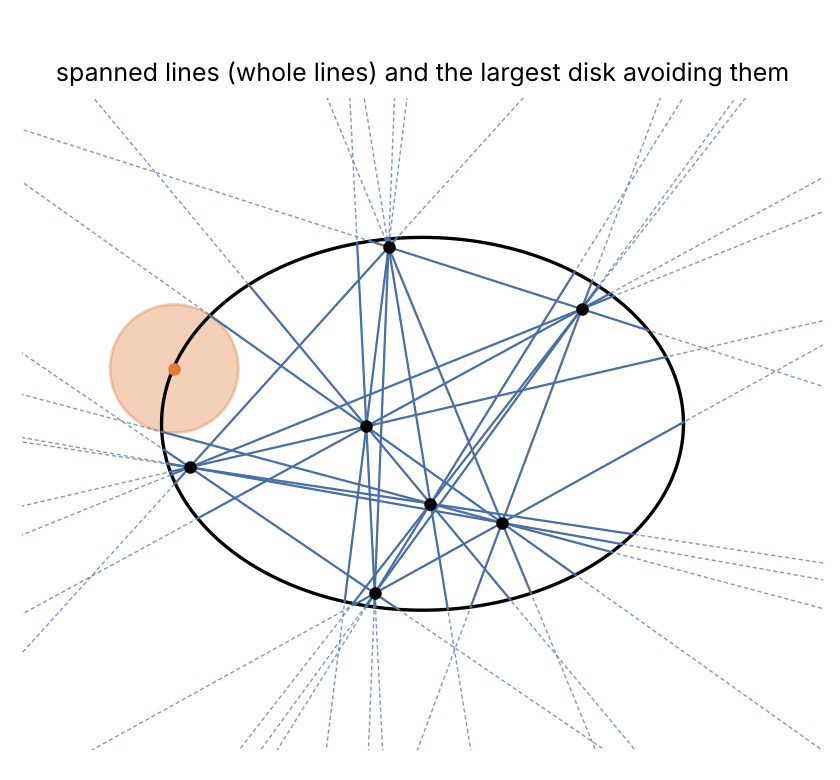
\includegraphics[width=0.55\textwidth]{figures/fig_lines_left.png}
\caption{Seven uniform points in an ellipse and the $21$ lines they span (dashed outside the ellipse). The largest open disk
centred in $\Omega$ that meets no line (it may leave $\Omega$) has radius $\rho^{(7)}_\Omega$. Floating-point illustration.}\label{fig:lines}
\end{figure}

\begin{corollary}\label{cor:ball}
Let $\Omega=\ball^d$ be the unit ball, $f$ uniform, $k=\frac{j(d+1)}2$, and $\mathrm B$ the Beta function. Then $h_{\ball^d}(z)$ depends
only on $|z|$ and is strictly decreasing in $|z|\in[0,1]$, so $M_f(\ball^d)$ is the unit sphere, and
\[
  c_{\ball^d}=\frac{(j+1)!\,d(j+1)}{2}\cdot\frac{\mathrm B(\frac a2,k+1)\,\mathrm B(\frac a2,\frac j2)}{\mathrm B(\frac a2,k+\frac j2)}.
\]
For planes ($j=2$) this is $18d/(d-2)$, e.g.\ $54$ in $\ball^3$; for lines it is $9\pi^2/8\approx11.10$ in the disk and $10$ in $\ball^3$.
\end{corollary}

By Theorem~\ref{thm:main}(b), for uniform points in a ball the points farthest from the spanned flats approach the boundary sphere;
for lines and uniform points in a square they approach the midpoints of the edges (Corollary~\ref{cor:square}).

\section{Geometric lemmas}\label{sec:geom}

This section collects estimates for the flat $F$ through $j+1$ independent points with density $f$. They hold for every
$j\in\{1,\dots,d-1\}$, and in Lemma~\ref{lem:share} we also use Lemma~\ref{lem:ig}(a) with $j-1$ in place of $j$. Let
$\Delta=\operatorname{diam}\Omega$, $f_+=\max_\Omega f$, $\kappa_k$ the volume of the unit ball of $\R^k$ ($\kappa_0=1$), and $\vol_k$
$k$-dimensional volume. In this section, constants $C,c$ (changing from line to line) and $K_0,C_0$ depend only on $d$, $j$, $\Delta$
and $f_+$.

The set $\mathcal G_j$ is open, its complement is Lebesgue-null (a zero set of a nonzero polynomial), and it is invariant under
permutations of $u_1,\dots,u_{j+1}$, as is $F(u)$. On $\mathcal G_j$ the orthogonal projection $P_{L(u)}$ onto the direction space
$L(u)$ of $F(u)$ is continuous (Gram--Schmidt applied to $u_2-u_1,\dots,u_{j+1}-u_1$), so $u\mapsto\dist(z,F(u))=|(I-P_{L(u)})(z-u_1)|$
is continuous on $\mathcal G_j$ for each $z$.

\paragraph{The integral-geometric representation.} Let $G(d,j)$ be the Grassmannian of $j$-dimensional linear subspaces,
identified with the orthogonal projections $P_L$ onto $L\in G(d,j)$, and $\nu_j$ its rotation-invariant probability measure; for
$L\in G(d,j)$ let $\pi_L=I-P_L$ be the orthogonal projection onto $L^\perp$, so that $\dist(z,L+p)=|p-\pi_Lz|$ for $p\in L^\perp$.
For $L\in G(d,j)$ and $p\in L^\perp$ let
\[
  G_L(p)=\int_{L^{j+1}}\prod_{i=1}^{j+1}f(\ell_i+p)\,\vol_j(\operatorname{conv}\{\ell_1,\dots,\ell_{j+1}\})^a\,d\ell ,
\]
with $d\ell$ Lebesgue measure on $L^{j+1}$. A set $\mathcal A$ of $j$-flats is \emph{measurable} if
$\{(L,p):p\in L^\perp,\ L+p\in\mathcal A\}$ is Borel.

\begin{lemma}[Representation]\label{lem:rep}
(a) The map $(L,p)\mapsto G_L(p)$ on $\{(L,p)\in G(d,j)\times\R^d:p\in L^\perp\}$ is Borel, $G_L\le G_{\max}:=f_+^{j+1}(\kappa_j\Delta^j)^{j+1+a}$, and
there is $b>0$ depending only on $d$ and $j$ such that for measurable $\mathcal A$,
\begin{equation}\label{eq:BPj}
  \Pr(F\in\mathcal A)=b\int_{G(d,j)}\int_{L^\perp}\Cone\{L+p\in\mathcal A\}\,G_L(p)\,dp\,\nu_j(dL).
\end{equation}
(b) For every $L$, $G_L$ vanishes outside the compact set $\pi_L(\Omega)$, and there is a Borel $\nu_j$-null set $\mathcal N\subseteq G(d,j)$
such that $G_L$ is continuous on $L^\perp$ for $L\notin\mathcal N$.
\end{lemma}

\begin{proof}
(a) The map is Borel by Appendix~\ref{app:meas}. The integrand of $G_L(p)$ vanishes unless every $\ell_i$ lies in
$K=\{\ell\in L:\ell+p\in\Omega\}$, a convex set of diameter $\le\Delta$, so $\vol_jK\le\kappa_j\Delta^j$ and
$\vol_j(\operatorname{conv}\{\ell_i\})\le\vol_jK$; this gives the bound. The affine Blaschke--Petkantschin formula
\cite[Theorem~7.2.7]{SW} with $q=j$ states that, for measurable $\varphi\ge0$ on $(\R^d)^{j+1}$,
\[
  \int_{(\R^d)^{j+1}}\varphi\,dx=b\int_{G(d,j)}\int_{L^\perp}\int_{(L+p)^{j+1}}\varphi\,\vol_j(\operatorname{conv}\{x_i\})^a\,dx\,dp\,\nu_j(dL),
\]
with a constant $b>0$ depending only on $d$ and $j$ (in \cite{SW} the measure on $j$-flats is normalized as the integral over
$L\in G(d,j)$, with $\nu_j$, of Lebesgue measure on $L^\perp$). Take $\varphi(x)=\prod_if(x_i)\Cone\{x\in\mathcal G_j,\ F(x)\in\mathcal A\}$ (Borel by
Appendix~\ref{app:meas}); its integral is $\Pr(F\in\mathcal A)$, as the complement of $\mathcal G_j$ is null. On $(L+p)^{j+1}$ every
tuple of positive weight spans $L+p$, and $x_i=\ell_i+p$ gives \eqref{eq:BPj}. (The value of $b$ is never taken from
\cite{SW}; where it is needed, it is determined by applying \eqref{eq:BPj} to the set of all $j$-flats.)

(b) The integrand of $G_L(p)$ vanishes unless $\ell_1+p\in\Omega$, and then $p=\pi_L(\ell_1+p)\in\pi_L(\Omega)$. The second is proved in Appendix~\ref{app:meas}, using a theorem of Ewald,
Larman and Rogers on the directions of segments in the boundary of a convex body \cite{ELR}.
\end{proof}

\begin{lemma}[Spanned flats]\label{lem:ig}
(a) For $z\in\R^d$ and $t>0$, $\Pr(\dist(z,F)<t)\le Ct^a$ and $\Pr(\dist(z,F)=t)=0$.
(b) For $x\ne y$ and $t>0$, $\Pr(\dist(x,F)<t,\ \dist(y,F)<t)\le Ct^{2a}|x-y|^{-a}$.
(c) As $t\to0$, $t^{-a}\Pr(\dist(z,F)<t)\to h_f(z)=b\kappa_a\int_{G(d,j)}G_L(\pi_Lz)\,\nu_j(dL)$ uniformly on compact subsets of $\R^d$,
and $h_f$ is continuous and positive on $\R^d$.
\end{lemma}

\begin{proof}
(a) In \eqref{eq:BPj}, $G_L\le G_{\max}$, and the sets $\{p\in L^\perp:|p-\pi_Lz|<t\}$ and $\{|p-\pi_Lz|=t\}$ have measure $\kappa_at^a$ and
$0$.

(b) Both events force $|\pi_L(x-y)|<2t$ and put $p$ in a ball of $L^\perp$ of radius $t$, of measure $\kappa_at^a$. For $\nu_j$-uniform
$L$ and a unit vector $e$, $|\pi_Le|^2$ has the law of the sum of $a$ squared coordinates of a uniform unit vector of $\R^d$ (by
rotation invariance), i.e.\ the Beta$(\frac a2,\frac j2)$ law; its density is at most $Cx^{a/2-1}$ on $[0,\frac12]$, so its
distribution function is at most $Cx^{a/2}$ for all $x\ge0$ (for $x\ge1$ it is $1\le x^{a/2}$), and $\nu_j\{L:|\pi_Le|<s\}\le Cs^a$. With $e=(x-y)/|x-y|$ and $s=2t/|x-y|$,
\eqref{eq:BPj} gives the bound.

(c) Define $h_f$ by the integral; $L\mapsto G_L(\pi_Lz)$ is Borel by Lemma~\ref{lem:rep}(a), as $L\mapsto(L,\pi_Lz)$ is continuous, and so
are the inner integrals below, by Tonelli. Let $t_n>0$, $t_n\to0$ and $z_n\to z$. For $L\notin\mathcal N$ (Lemma~\ref{lem:rep}(b)), $G_L$ is continuous at
$\pi_Lz$, so $t_n^{-a}\int_{|p-\pi_Lz_n|<t_n}G_L(p)\,dp\to\kappa_aG_L(\pi_Lz)$ and $G_L(\pi_Lz_n)\to G_L(\pi_Lz)$; all these are at most
$\max(1,\kappa_a)G_{\max}$. By \eqref{eq:BPj} and dominated convergence, $t_n^{-a}\Pr(\dist(z_n,F)<t_n)\to h_f(z)$ and $h_f(z_n)\to h_f(z)$. So $h_f$ is
continuous, the limit exists, and the convergence is uniform on compact sets: otherwise there are $\eta>0$, $t_n\to0$ and $z_n$ in a
compact set with $|t_n^{-a}\Pr(\dist(z_n,F)<t_n)-h_f(z_n)|\ge\eta$, and a convergent subsequence of $(z_n)$ gives a contradiction.

For positivity, fix $z$. Since $\partial\Omega$ is null and $\int f=1$, there are a ball $B(o,r_0)\subseteq\Omega$ and $f_->0$ with $f\ge f_-$
on it ($f$ is continuous on $\Omega$). Let $L_0\in G(d,j)$ contain $o-z$. On a neighbourhood $\mathcal V$ of $L_0$, $\dist(o,L+\pi_Lz)=|\pi_L(o-z)|<r_0/2$,
so $(L+\pi_Lz)\cap B(o,r_0)$ contains a $j$-ball of radius $r_0/2$ on which $f\ge f_-$, and $G_L(\pi_Lz)>0$. Finitely many rotations of
$\mathcal V$ cover the compact homogeneous space $G(d,j)$, so $\nu_j(\mathcal V)>0$ and $h_f(z)>0$.
\end{proof}

\begin{lemma}[Adding a point]\label{lem:flat}
There is $K_0\ge1$ such that for every $(j-1)$-flat $E$ meeting $\Omega$ (a point of $\Omega$ if $j=1$), every $z\in\R^d$ with
$D=\dist(z,E)>0$, $U$ with density $f$, and all $r>0$, $\Pr(\dist(z,\Caff(E,U))\le r)\le K_0(r/D)^a$.
\end{lemma}

\begin{proof}
If $r\ge D$ the bound holds as $K_0\ge1$; let $r<D$. Let $W$ be the orthogonal complement of the direction space of $E$, so
$\dim W=a+1$, and $\Cpr$ the orthogonal projection onto $W$; $\Cpr E=\{e_0\}$ is a point and $|\Cpr z-e_0|=D$. If $\Cpr U\ne e_0$ (the event
$U\in E$ is null), $\Caff(E,U)$ is the preimage under $\Cpr$ of the line through $e_0$ and $\Cpr U$, so $\dist(z,\Caff(E,U))=D\sin\varphi$,
with $\varphi$ the angle between that line and $\Cpr z-e_0$; so $\dist\le r$ forces $\varphi\le\chi:=\arcsin(r/D)\le\pi r/(2D)$. Fix $e\in E\cap\Omega$.
Then $\Cpr(U-e)$ lies in the double cone in $W$ of half-angle $\chi$ and radius $\Delta$ about the line through $0$ and $\Cpr z-e_0$, which
has volume at most $C\Delta^{a+1}\chi^a$, and the component of $U-e$ in the direction space of $E$ lies in a $(j-1)$-ball of radius $\Delta$.
As the density of $U$ is at most $f_+$, Fubini gives $\Pr(\dist(z,\Caff(E,U))\le r)\le C(r/D)^a$, and $K_0=\max(1,C)$ works.
\end{proof}

For a $(j+1)$-tuple $u$ and $z\in\R^d$ let $\sigma_z(u)$ be the smallest distance from $z$ to the affine hull of $j$ of the entries
of $u$ (for $j=1$, $\sigma_z(u)=\min_i|z-u_i|$).

\begin{lemma}[Sub-tuples]\label{lem:share}
Let $1\le i\le j$, and let $S = (U_1, \dots, U_i)$, $V = (U_{i+1}, \dots, U_{j+1})$, $V' = (U'_{i+1}, \dots, U'_{j+1})$ be
independent tuples of independent points with density $f$; $F_{S,V}$ is the flat through the entries of $S$ and $V$. For
$z,z'\in\R^d$ and $\eps,\tau>0$ let
\[
  P=\Pr\bigl(\dist(z,F_{S,V})<\eps,\ \sigma_z(S,V)>\tau,\ \dist(z',F_{S,V'})<\eps,\ \sigma_{z'}(S,V')>\tau\bigr),
\]
and let $P^\circ$ be the same probability without the two conditions on $\sigma$.
(a) If $a=1$ and $0<\eps\le\frac12$, then $P\le P^\circ\le C\eps^2(1+\log(1/\eps))$.
(b) If $a\ge2$, then $P\le C\eps^{2a}\tau^{1-a}$.
(c) For $z\in\R^d$ and $\eps,\tau>0$, $\Pr(\dist(z,F)<\eps,\ \sigma_z(U_1,\dots,U_{j+1})\le\tau)\le C\eps^a\tau$.
\end{lemma}

\begin{proof}
Let $D$ be the distance from a point $z$ to the affine hull of $j$ independent points with density $f$. Then
$\Pr(D\le s)\le C_0s^{a+1}$ for $s>0$, with $C_0\ge1$: for $j=1$, $D=|z-U_1|$ and $\Pr(D\le s)\le f_+\kappa_ds^d$; for $j\ge2$ this is
Lemma~\ref{lem:ig}(a) with $j-1$ in place of $j$. In particular $D>0$ almost surely.

(a), (b) Given $S$ the two events are independent, so $P\le(\E q_z(S)^2)^{1/2}(\E q_{z'}(S)^2)^{1/2}$, where $q_z(S)$ is the conditional
probability of the first, and it suffices to bound $\E q_z(S)^2$ uniformly in $z$. Write $V=(V_1,U_{j+1})$ ($V_1$ is empty if $i=j$), and let $D=\dist(z,\Caff(S,V_1))$, the
distance to the flat of a $j$-sub-tuple (so $D$ has the law above). Given $(S,V_1)$, the first event has probability at most
$\min(1,K_0(\eps/D)^a)$ by Lemma~\ref{lem:flat} (almost surely $\Caff(S,V_1)$ is a $(j-1)$-flat containing $U_1\in\Omega$, and $U_{j+1}$
is independent of $(S,V_1)$), and it requires $D>\tau$ (we drop the other conditions in $\sigma_z>\tau$). By conditional Jensen,
$\E q_z^2\le\E[\min(1,K_0(\eps/D)^a)^2\Cone\{D>\tau\}]$; without the condition on $\sigma$, the same holds without $\Cone\{D>\tau\}$.
If $a=1$, then with $c=C_0K_0^2\eps^2\ge\eps^2$,
\[
  \E\min(1,K_0^2\eps^2D^{-2})=\int_0^1\Pr(D<K_0\eps u^{-1/2})\,du\le\int_0^1\min(1,c/u)\,du\le c(1+\log^+(1/c))\le C_0K_0^2\eps^2(1+2\log(1/\eps)).
\]
If $a\ge2$, then as $\frac{a+1}{2a}<1$,
\[
  \E\bigl[D^{-2a}\Cone\{D>\tau\}\bigr]\le\int_0^{\tau^{-2a}}\Pr\bigl(D<s^{-1/(2a)}\bigr)\,ds\le C_0\int_0^{\tau^{-2a}}s^{-\frac{a+1}{2a}}\,ds=\frac{2a}{a-1}C_0\,\tau^{1-a},
\]
so $\E q_z^2\le\frac{2a}{a-1}K_0^2C_0\eps^{2a}\tau^{1-a}$.

(c) By exchangeability it suffices to bound $\Pr(\dist(z,F)<\eps,\ D\le\tau)$ with $D=\dist(z,\Caff(U_1,\dots,U_j))$, and multiply by $j+1$.
By Lemma~\ref{lem:flat} given $U_1,\dots,U_j$ (as in (a), (b)), this is at most
\[
  K_0\eps^a\E\bigl[D^{-a}\Cone\{D\le\tau\}\bigr]\le K_0\eps^a\Bigl(\tau^{-a}\Pr(D\le\tau)+\int_{\tau^{-a}}^\infty\Pr(D<s^{-1/a})\,ds\Bigr)\le(1+a)K_0C_0\eps^a\tau.
  \qedhere
\]
\end{proof}

\section{Proof of Theorem~\ref{thm:main}}\label{sec:proof}

\begin{thmH}[{\cite{Harris}; see \cite[Section~6.3]{AS}}]
If $I_1,\dots,I_M$ are independent $\{0,1\}$-valued and $A_1, \dots, A_r$ are decreasing events determined by $I_1,\dots,I_M$ (preserved by changing
some $I_k$ from $1$ to $0$), then $\Pr(A_1 \cap \dots \cap A_r) \ge \prod_i \Pr(A_i)$. (The cited case is $r=2$; the
general case follows by induction, as an intersection of decreasing events is decreasing.)
\end{thmH}

\begin{thmJ}[{\cite{Janson}; see \cite[Section~8.1]{AS}}]
Let $R$ contain each element $k$ of a finite set independently with probability $p_k$, let $S_1, \dots, S_r$ be subsets,
$A_i = \{S_i \subseteq R\}$, $\bar\mu = \sum_i\Pr(A_i)$ and $\bar{\mathcal D} = \sum\Pr(A_i \cap A_{i'})$ over ordered pairs $i \ne i'$ with
$S_i \cap S_{i'} \ne \emptyset$. Then $\Pr(\text{no }A_i) \le e^{-\bar\mu+\bar{\mathcal D}}$ (a weak form of the inequality in \cite{AS}).
\end{thmJ}

\paragraph{Set-up.} In this section constants $C,c$ may also depend on $\Omega$, $f$, the covered set and the parameters fixed in
the set-up or at the start of a proof, but never on $n$ or on the points $z,z',x,y$. Given $c_0>0$, $\vartheta\in(0,1)$ and a sign,
let
\[
  \eps^a=\frac{c_0\log n}{n^{j+1}},\qquad \tau_n=n^{j/a}\eps\ \ \Bigl(\text{so }\tau_n^a=\frac{c_0\log n}n\Bigr),\qquad\delta_n=n^{-1/a}(\log n)^3,\qquad\lambda=(1\mp\vartheta)n.
\]
Let $N \sim \mathrm{Poisson}(\lambda)$ be independent of the $X_i$ (on a product extension of the probability space), and
$\Pi = \{X_1, \dots, X_N\}$, a Poisson process with intensity measure $\lambda f(x)\,dx$. For Borel $\mathcal E\subseteq(\R^d)^{j+1}$ let
$\bar P(\mathcal E)=\frac{\lambda^{j+1}}{(j+1)!}\int_{\mathcal E}\prod_if(u_i)\,du$. For $z\in\R^d$ let $E_z$ be the event that no $j+1$ points of $\Pi$
span a $j$-flat $F'$ with $\dist(z,F')<\eps$ ($z$ is uncovered), and
\[
  \mu_z=\bar P\bigl(\{u\in\mathcal G_j:\dist(z,F(u))<\eps\}\bigr)=\frac{\lambda^{j+1}}{(j+1)!}\Pr(\dist(z,F)<\eps).
\]
Let $\mathcal T_z$ be the set of $u\in\mathcal G_j$ with $\dist(z,F(u))<\eps$ and, if $a\ge2$, $\sigma_z(u)>\tau_n$. It is open (the distance
from $z$ to the affine hull of a sub-tuple is continuous where that sub-tuple is affinely independent, as it is on $\mathcal G_j$)
and invariant under permutations of the coordinates. Adding points adds flats, so on $\{N\le n\}$ every flat spanned by $\Pi$ is
spanned by $X_1,\dots,X_n$, and on $\{N\ge n\}$ the converse holds; by Chebyshev's inequality,
$\Pr(N>n)\le(\vartheta^2n)^{-1}$ if $\lambda=(1-\vartheta)n$ and $\Pr(N<n)\le2(\vartheta^2n)^{-1}$ if $\lambda=(1+\vartheta)n$.

\paragraph{Why a restriction is used.} For $j<d/2$ and without the condition on $\sigma_z$, pairs of flats sharing one sample
point near $z$ contribute at least of order $(\log n)^{d/(d-j)}$ to Janson's pair term, more than the mean $\asymp\log n$: the
$\asymp n\eps^d$ sample points within $\eps$ of $z$ lie on $\asymp n^{2j}$ such pairs each, giving
$\asymp n^{j(d-2j-1)/(d-j)}(\log n)^{d/(d-j)}$, and $j(d-2j-1)\ge0$ exactly when $j<d/2$. For $d/2\le j\le d-2$ the restriction is not
needed heuristically, but the bound of Lemma~\ref{lem:share} without it would involve $\E D^{-2a}$, which is infinite for $a\ge2$ (for
$j\ge2$, $\Pr(D\le s)$ is of order $s^{a+1}$ by Lemma~\ref{lem:ig}(c) with $j-1$ in place of $j$); the restriction costs nothing.

\begin{lemma}[One and two points]\label{lem:poisson}
For $z,z'\in\R^d$, (a) $\Pr(E_z)\ge e^{-\mu_z}$, and (b)
\[
  \Pr(E_z\cap E_{z'})\le\exp\bigl(-\bar P(\mathcal T_z\cup\mathcal T_{z'})+\mathcal D\bigr),\qquad
  \mathcal D=\sum_{i=1}^{j}\lambda^{2(j+1)-i}\sum_{(y_1,y_2)\in\{z,z'\}^2}\Pr\bigl((S,V)\in\mathcal T_{y_1},\ (S,V')\in\mathcal T_{y_2}\bigr),
\]
with $S,V,V'$ as in Lemma~\ref{lem:share} (for this $i$), and four terms in the inner sum also when $z=z'$.
\end{lemma}

\begin{proof}
We discretize $\Omega$ into cells of diameter $\eta$ and let $\eta\to0$ with $n$ fixed. Let $0<\eta\le1$. The \emph{cells} are the
nonempty sets $Q_k = \Omega \cap ((\eta/\sqrt d)(k+[0,1)^d))$, $k\in\Z^d$; they partition $\Omega$ and have diameter $\le\eta$ and volume
$\le\eta^d$. The numbers $N_k$ of points of $\Pi$ in $Q_k$ are independent $\mathrm{Poisson}(\lambda w_k)$ with $w_k=\int_{Q_k}f\le f_+\eta^d$, so
$I_k = \Cone\{N_k \ge 1\}$ has $p_k = \Pr(I_k = 1)=1-e^{-\lambda w_k}\in[\lambda w_k(1 - \lambda f_+\eta^d),\lambda w_k]$, and the event $\mathrm{Two}$
that some cell holds at least two points of $\Pi$ has $\Pr(\mathrm{Two}) \le\sum_k(\lambda w_k)^2\le \lambda^2f_+\eta^d$. A \emph{cell set}
is a set $\mathcal C$ of $j+1$ cell indices; it is \emph{occupied} if $I_k=1$ for all $k\in\mathcal C$. Let $w(\mathcal C)=\prod_{k\in\mathcal C}w_k$ and
let $Q_{\mathcal C}$ be the set of $u\in\Omega^{j+1}$ with exactly one coordinate in each $Q_k$, $k\in\mathcal C$; so $\bar P(Q_{\mathcal C})=\lambda^{j+1}w(\mathcal C)$, and
the $Q_{\mathcal C}$ are pairwise disjoint. For a family $\CB$ of cell sets let $\mathcal U(\CB)=\bigcup_{\mathcal C\in\CB}Q_{\mathcal C}$, so
$\bar P(\mathcal U(\CB))=\lambda^{j+1}\sum_{\mathcal C\in\CB}w(\mathcal C)$. If $u\in\Omega^{j+1}\cap\mathcal G_j$, its coordinates are distinct, so for small
$\eta$ they lie in distinct cells, forming a cell set $\mathcal C$ with $u\in Q_{\mathcal C}$, and every $u'\in Q_{\mathcal C}$ is, after a permutation of
its coordinates (which changes neither $\mathcal G_j$ nor $F$), within $\eta$ of $u$ in each coordinate.

(a) Let $\CB_+$ be the family of cell sets $\mathcal C$ such that some $u\in Q_{\mathcal C}\cap\mathcal G_j$ has $\dist(z,F(u))<\eps$. Off $\mathrm{Two}$ (and as
$\Pi\subset\Omega$ almost surely), $j+1$ points of $\Pi$ spanning a flat within $\eps$ of $z$ lie in distinct cells, which form a set in
$\CB_+$. So $E_z$ contains the event that no set in $\CB_+$ is occupied, minus $\mathrm{Two}$. The events that a given set $\mathcal C$ is not
occupied are decreasing, with probability $1-q_{\mathcal C}$, $q_{\mathcal C}=\prod_{k\in\mathcal C}p_k\le\lambda^{j+1}w(\mathcal C)\le(\lambda f_+\eta^d)^{j+1}$. For $\eta$
so small that $(\lambda f_+\eta^d)^{j+1}\le\frac12$, Harris's inequality and $\log(1-q)\ge-q(1+q)$ for $0\le q\le\frac12$ give
\[
  \Pr(E_z)\ge\prod_{\mathcal C\in\CB_+}(1-q_{\mathcal C})-\Pr(\mathrm{Two})\ge\exp\Bigl(-\bigl(1+(\lambda f_+\eta^d)^{j+1}\bigr)\bar P(\mathcal U(\CB_+))\Bigr)-\lambda^2f_+\eta^d.
\]
Let $u\in\Omega^{j+1}\cap\mathcal G_j$ with $\dist(z,F(u))>\eps$. As $\mathcal G_j$ is open and $\dist(z,F(\cdot))$ is continuous on it, for small $\eta$
every $u'\in Q_{\mathcal C}$ ($\mathcal C$ as above) lies in $\mathcal G_j$ and has $\dist(z,F(u'))>\eps$, so $\mathcal C\notin\CB_+$ and $u\notin\mathcal U(\CB_+)$. The
remaining $u\in\Omega^{j+1}$ with $\dist(z,F(u))\ge\eps$ form a null set (the complement of $\mathcal G_j$ is null, and
Lemma~\ref{lem:ig}(a)). So $\limsup_{\eta\to0}\Cone_{\mathcal U(\CB_+)}\le\Cone\{\dist(z,F(\cdot))<\eps\}$ for $\bar P$-almost every $u$, and by
the reverse Fatou lemma ($\bar P$ is finite and $0\le\Cone_{\mathcal U(\CB_+)}\le1$) $\limsup_{\eta\to0}\bar P(\mathcal U(\CB_+))\le\mu_z$; letting $\eta\to0$ gives (a).

(b) For $y\in\{z,z'\}$ let $\CB_y=\{\mathcal C:Q_{\mathcal C}\subseteq\mathcal T_y\}$ and $\CB=\CB_z\cup\CB_{z'}$. If a set in $\CB_y$ is occupied, any choice of one
point of $\Pi$ per cell is a tuple in $\mathcal T_y$, which spans a flat within $\eps$ of $y$; so $E_z\cap E_{z'}$ is contained in the event
that no set in $\CB$ is occupied. Janson's inequality with $R=\{k:I_k=1\}$ and the events $A_{\mathcal C}=\{\mathcal C\subseteq R\}$, $\mathcal C\in\CB$, bounds
its probability by $\exp(-\bar\mu+\bar{\mathcal D}_\eta)$, where, for $\lambda f_+\eta^d\le1$, $\bar\mu=\sum_{\mathcal C\in\CB}q_{\mathcal C}\ge(1-\lambda f_+\eta^d)^{j+1}\bar P(\mathcal U(\CB))$,
and $\bar{\mathcal D}_\eta$ is the pair term. For $u\in(\mathcal T_z\cup\mathcal T_{z'})\cap\Omega^{j+1}$, say $u\in\mathcal T_y$, $Q_{\mathcal C}\subseteq\mathcal T_y$ for small $\eta$, as $\mathcal T_y$ is
open and permutation invariant; so $\liminf_{\eta\to0}\Cone_{\mathcal U(\CB)}\ge\Cone_{\mathcal T_z\cup\mathcal T_{z'}}$ on $\Omega^{j+1}$, and by Fatou's lemma
$\liminf_{\eta\to0}\bar P(\mathcal U(\CB))\ge\bar P(\mathcal T_z\cup\mathcal T_{z'})$. An ordered pair $(\mathcal C,\mathcal C')$ counted in $\bar{\mathcal D}_\eta$ has
$|\mathcal C\cap\mathcal C'|=i\in[1,j]$ and $\Pr(A_{\mathcal C}\cap A_{\mathcal C'})\le\lambda^{2(j+1)-i}\prod_{k\in\mathcal C\cup\mathcal C'}w_k$. Fix $i$, $y_1,y_2\in\{z,z'\}$ and the
pairs with $\mathcal C\in\CB_{y_1}$, $\mathcal C'\in\CB_{y_2}$ (a pair may be counted for several choices, which only increases the bound). Listing the
indices of $\mathcal C\cap\mathcal C'$, $\mathcal C\setminus\mathcal C'$ and $\mathcal C'\setminus\mathcal C$, each in increasing lexicographic order, gives products of
cells in $\Omega^{2(j+1)-i}$; these are disjoint (a point determines its cell), have $f^{\otimes(2(j+1)-i)}$-measure $\prod_{\mathcal C\cup\mathcal C'}w_k$,
and lie in $\{(s,v,v'):(s,v)\in\mathcal T_{y_1},\ (s,v')\in\mathcal T_{y_2}\}$, as $Q_{\mathcal C}\subseteq\mathcal T_{y_1}$ and $Q_{\mathcal C'}\subseteq\mathcal T_{y_2}$. Summing,
$\bar{\mathcal D}_\eta\le\mathcal D$ for every $\eta$; let $\eta\to0$.
\end{proof}

\begin{lemma}[Uncovered points]\label{lem:fam}
Here $\lambda=(1\mp\vartheta)n$, so $1\le\lambda\le2n$ for large $n$. For large $n$ and all $z,z'\in\R^d$,
\[
  e^{-\mu_z}\le\Pr(E_z)\le e^{-\mu_z+C\delta_n},\qquad
  \Pr(E_z\cap E_{z'})\le\exp\Bigl(-\mu_z-\mu_{z'}+C\delta_n+\frac{\lambda^{j+1}}{(j+1)!}\Pr\bigl(\dist(z,F)<\eps,\ \dist(z',F)<\eps\bigr)\Bigr).
\]
\end{lemma}

\begin{proof}
We show (i) $\mu_y-\bar P(\mathcal T_y)\le C\delta_n$ for all $y$, and (ii) $\mathcal D\le C\delta_n$. Then
$\bar P(\mathcal T_z\cup\mathcal T_{z'})=\bar P(\mathcal T_z)+\bar P(\mathcal T_{z'})-\bar P(\mathcal T_z\cap\mathcal T_{z'})$ and
$\bar P(\mathcal T_z\cap\mathcal T_{z'})\le\frac{\lambda^{j+1}}{(j+1)!}\Pr(\dist(z,F)<\eps,\ \dist(z',F)<\eps)$, so Lemma~\ref{lem:poisson} gives the
claims (the upper bound for $\Pr(E_z)$ with $z'=z$).

(i) For $a=1$ the left side is $0$. For $a\ge2$, a tuple counted in $\mu_y$ but not in $\mathcal T_y$ has $\sigma_y\le\tau_n$, so by
Lemma~\ref{lem:share}(c) the left side is at most $C\lambda^{j+1}\eps^a\tau_n\le Cn^{j+1}\eps^a\tau_n=C(\log n)^{1+1/a}n^{-1/a}\le C\delta_n$ (as $1+1/a\le3$).
(ii) As $\lambda\ge1$, $\lambda^{2(j+1)-i}\le(2n)^{2j+1}$. A pair counted in $\mathcal D$ satisfies the events defining $P^\circ$ (if $a=1$) or $P$ (if $a\ge2$) in
Lemma~\ref{lem:share}, with $(z,z')=(y_1,y_2)$ and $\tau=\tau_n$. For $a=1$, Lemma~\ref{lem:share}(a) (with $\eps\le\frac12$ for large $n$) and $\log(1/\eps)\le C\log n$
give $\mathcal D\le Cn^{2j+1}\eps^2\log n=C(\log n)^3/n$. For $a\ge2$, Lemma~\ref{lem:share}(b) gives
$\mathcal D\le Cn^{2j+1}\eps^{2a}\tau_n^{1-a}=Cn^{j+1+j/a}\eps^{a+1}=C(\log n)^{1+1/a}n^{-1/a}\le C\delta_n$.
\end{proof}

\begin{proposition}[Upper bound]\label{prop:upper}
Let $A\subset\R^d$ be nonempty and compact. For every $\xi>0$ there are $C,c>0$ with
$\Pr\bigl(n^{j+1}(\rho_A^{(n)})^a/\log n>c_f(A)+\xi\bigr)\le Cn^{-c}$ for all $n\ge j+1$.
\end{proposition}

\begin{proof}
Let $m=m_f(A)$ and $c_+=c_f(A)+\xi/2$, and fix $\eta\in(0,1]$ with $(1+\eta)^ac_+\le c_f(A)+\xi$. Since $mc_+/(j+1)!=d(j+1)/a+m\xi/(2(j+1)!)$,
we can fix $\vartheta,\zeta\in(0,1)$ with $\zeta<m$ and $(1-\vartheta)^{j+1}(m-\zeta)c_+/(j+1)!\ge d(j+1)/a+2\zeta$. Use the set-up with $c_0=c_+$ and
$\lambda=(1-\vartheta)n$; it suffices to take $n$ large (then enlarge $C$).

\emph{One point.} By Lemma~\ref{lem:ig}(c) and the uniform continuity of $h_f$ on the compact set $A^{(1)}=\{x:\dist(x,A)\le1\}$,
there are $t_0,r_A\in(0,1]$ with $\Pr(\dist(z,F)<t)\ge(m-\zeta)t^a$ whenever $\dist(z,A)\le r_A$ and $t\le t_0$. For large $n$, $\eps\le t_0$, so
for such $z$, $\mu_z\ge(1-\vartheta)^{j+1}n^{j+1}(m-\zeta)\eps^a/(j+1)!\ge(d(j+1)/a+2\zeta)\log n$, and by Lemma~\ref{lem:fam},
$\Pr(E_z)\le e^{C\delta_n}n^{-d(j+1)/a-2\zeta}\le2n^{-d(j+1)/a-2\zeta}$.

\emph{Net.} Let $\mathcal M$ be the set of points of $(\eta\eps/\sqrt d)\Z^d$ within $\eta\eps/2$ of $A$. Every $x\in A$ is within $\eta\eps/2$
of a point of the grid, which is in $\mathcal M$. For large $n$, $\eta\eps/2\le r_A$ and $3\eta\eps/2\le1$, so the disjoint cubes $x+[0,\eta\eps/\sqrt d)^d$,
$x\in\mathcal M$ (which lie within $\eta\eps/2+\eta\eps$ of $A$), lie in $A^{(1)}$, and $|\mathcal M|\le|A^{(1)}|(\sqrt d/(\eta\eps))^d\le Cn^{d(j+1)/a}$, as
$\eps^{-d}=(n^{j+1}/(c_+\log n))^{d/a}$. Hence the union of the $E_z$, $z\in\mathcal M$,
has probability at most $Cn^{-2\zeta}$, and off this event every point of $A$ is at distance $<(1+\eta)\eps$ from a flat spanned by
points of $\Pi$; and $(1+\eta)^a\eps^a\le(c_f(A)+\xi)\log n/n^{j+1}$.

\emph{De-Poissonization.} On $\{N\le n\}$ these flats are spanned by $X_1,\dots,X_n$, so the probability in the statement is at most
$Cn^{-2\zeta}+(\vartheta^2n)^{-1}\le Cn^{-c}$.
\end{proof}

\begin{proposition}[Lower bound]\label{prop:lower}
Let $\Lambda\subset\R^d$ be nonempty, compact and the closure of its interior. For every $\xi\in(0,c_f(\Lambda))$ there are $C,c>0$ with
$\Pr\bigl(n^{j+1}(\rho_\Lambda^{(n)})^a/\log n<c_f(\Lambda)-\xi\bigr)\le Cn^{-c}$ for all $n\ge j+1$.
\end{proposition}

\begin{proof}
Let $m=m_f(\Lambda)$ and $c_-=c_f(\Lambda)-\xi$. Since $mc_-/(j+1)!=d(j+1)/a-m\xi/(j+1)!$, we can fix $\vartheta,\zeta\in(0,1)$ with
$(1+\vartheta)^{j+1}(m+\zeta)c_-/(j+1)!\le d(j+1)/a-3\zeta$. Use the set-up with $c_0=c_-$ and $\lambda=(1+\vartheta)n$; it suffices to take $n$ large.

\emph{Test points.} Let $z_0\in\Lambda$ with $h_f(z_0)=m$. By Lemma~\ref{lem:ig}(c) (uniform convergence near $z_0$, and continuity of
$h_f$ at $z_0$) there are $r>0$ and $t_1>0$ with $\Pr(\dist(z,F)<t)\le(m+\zeta)t^a$ for $z\in B(z_0,r)$ and $t\le t_1$. As $\Lambda$ is the
closure of its interior, there is a ball $B(z_1,r_1)\subseteq\Lambda\cap B(z_0,r)$ with $r_1>0$. Let $s_n=\eps n^{\zeta/d}$, which tends to
$0$ since $\zeta/d<1/d<(j+1)/a$, and $\mathcal Z=s_n\Z^d\cap B(z_1,r_1)$. Distinct points of $\mathcal Z$ are $\ge s_n$ apart, and once $s_n\sqrt d\le r_1/2$
the cubes $x+[0,s_n)^d$, $x\in\mathcal Z$, cover $B(z_1,r_1/2)$, so $|\mathcal Z|\ge cs_n^{-d}$. For large $n$, $\eps\le t_1$, and for $z\in\mathcal Z$,
$\mu_z\le(1+\vartheta)^{j+1}n^{j+1}(m+\zeta)\eps^a/(j+1)!\le(d(j+1)/a-3\zeta)\log n$, so $\Pr(E_z)\ge e^{-\mu_z}\ge n^{-d(j+1)/a+3\zeta}$ by
Lemma~\ref{lem:fam}.

\emph{Pairs.} Let $x\ne y$ in $\mathcal Z$. As $|x-y|\ge s_n$, Lemma~\ref{lem:ig}(b) gives
$\frac{\lambda^{j+1}}{(j+1)!}\Pr(\dist(x,F)<\eps,\ \dist(y,F)<\eps)\le Cn^{j+1}\eps^{2a}s_n^{-a}=Cc_-\log n\cdot n^{-a\zeta/d}\le n^{-a\zeta/(2d)}$ for large $n$.
With $\delta_n\le n^{-1/(2a)}$, Lemma~\ref{lem:fam} gives, with $c_2=\min(\frac1{2a},\frac{a\zeta}{2d})$ and $C$ independent of $x,y\in\mathcal Z$,
\[
  \Pr(E_x \cap E_y) \le e^{Cn^{-c_2}}e^{-\mu_x-\mu_y}\le\bigl(1+Cn^{-c_2}\bigr)\Pr(E_x)\Pr(E_y).
\]

\emph{Second moment.} Let $Y = \sum_{z \in\mathcal Z}\Cone_{E_z}$. As $s_n^{-d}=\eps^{-d}n^{-\zeta}=(n^{j+1}/(c_-\log n))^{d/a}n^{-\zeta}$,
$\E Y\ge cs_n^{-d}n^{-d(j+1)/a+3\zeta}\ge cn^{2\zeta}(\log n)^{-d/a}\ge n^\zeta$ for large $n$. By the pair bound,
\[
  \operatorname{Var}Y\le\sum_z\Pr(E_z)+\sum_{x\ne y}\bigl(\Pr(E_x\cap E_y)-\Pr(E_x)\Pr(E_y)\bigr)\le\E Y+Cn^{-c_2}(\E Y)^2,
\]
so by Chebyshev's inequality $\Pr(Y = 0) \le 1/\E Y + Cn^{-c_2}\le n^{-\zeta}+Cn^{-c_2}$.

\emph{Conclusion.} On $\{N\ge n\}\cap\{Y>0\}$ some $z\in\mathcal Z\subseteq\Lambda$ is at distance $\ge\eps$ from every flat spanned by points of
$\Pi\supseteq\{X_1,\dots,X_n\}$, so $\rho_\Lambda^{(n)}\ge\eps$, i.e.\ $n^{j+1}(\rho_\Lambda^{(n)})^a/\log n\ge c_-$. Hence the probability in the
statement is at most $\Pr(Y=0)+\Pr(N<n)\le Cn^{-c}$ with $c=\min(\zeta,c_2)$.
\end{proof}

\begin{proof}[Proof of Theorem~\ref{thm:main}]
(a) Adding points only adds flats, so $\rho_\Lambda^{(n)}$ is nonincreasing in $n$. Write $R_n=n^{j+1}(\rho_\Lambda^{(n)})^a/\log n$ and fix
$\xi\in(0,c_f(\Lambda))$. By Propositions~\ref{prop:upper} (with $A=\Lambda$) and~\ref{prop:lower} there are $C,c>0$ with
$\Pr(|R_n-c_f(\Lambda)|>\xi)\le Cn^{-c}$ for $n\ge j+1$. Let $n_k=\lceil k^{2/c}\rceil$. Then $\sum_k\Pr(|R_{n_k}-c_f(\Lambda)|>\xi)<\infty$ (over
$k$ with $n_k\ge j+1$), so by Borel--Cantelli, almost surely $|R_{n_k}-c_f(\Lambda)|\le\xi$ for all large $k$. For $n\ge n_1$ let
$k=k(n)=\max\{k:n_k\le n\}$; then $n\in[n_k,n_{k+1}]$ and $k(n)\to\infty$, and the monotonicity of $\rho_\Lambda^{(\cdot)}$ and of $\log$
gives
\[
  \Bigl(\frac{n_k}{n_{k+1}}\Bigr)^{j+1}R_{n_{k+1}}\le R_n\le\Bigl(\frac{n_{k+1}}{n_k}\Bigr)^{j+1}R_{n_k}.
\]
As $n_{k+1}/n_k\to1$, almost surely $c_f(\Lambda)-\xi\le\liminf_nR_n\le\limsup_nR_n\le c_f(\Lambda)+\xi$. Let $\xi\to0$ along a sequence.

(b) Fix $s>0$ and let $A=\{x\in\Lambda:\dist(x,M_f(\Lambda))\ge s\}$; we may assume $A\ne\emptyset$. As $A$ is compact and disjoint from
$M_f(\Lambda)$, and $h_f$ is continuous, $m_f(A)>m_f(\Lambda)$, so $c_f(A)<c_f(\Lambda)$. Since $\rho_A^{(n)}$ is nonincreasing in $n$, the argument
of (a) with Proposition~\ref{prop:upper} for $A$ gives, almost surely, $\limsup_nn^{j+1}(\rho_A^{(n)})^a/\log n\le c_f(A)<c_f(\Lambda)$. Hence,
by (a), almost surely $\rho_A^{(n)}<\rho_\Lambda^{(n)}$ for all large $n$; then no maximizer $x$ in (b) lies in $A$, so the maximum in (b), attained as the set of maximizers is nonempty and compact, is
$<s$. Let $s\to0$ along a sequence.
\end{proof}

\section{Explicit constants and examples}\label{sec:examples}

We prove Corollary~\ref{cor:ball} and then treat lines in the plane. Since $h_{g\Omega}(gz)=h_\Omega(z)$ for isometries $g$ and
$h_{s\Omega}(sz)=s^{-a}h_\Omega(z)$ for $s>0$, $c_\Omega$ is invariant under isometries and $c_{s\Omega}=s^ac_\Omega$. The closed forms below were
also checked in exact (symbolic) arithmetic by \texttt{ball\_flats.py} in \cite{Repo}, which also tabulates further ball constants.

\begin{proof}[Proof of Corollary~\ref{cor:ball}]
Let $f=1/\kappa_d$ on $\ball^d$. For $L\in G(d,j)$ and $p\in L^\perp$ with $|p|<1$, $(L+p)\cap\ball^d$ is the $j$-ball of radius
$\varrho=(1-|p|^2)^{1/2}$ about $p$; substituting $\ell_i=\varrho w_i$ in the definition of $G_L(p)$ gives
$G_L(p)=\kappa_d^{-(j+1)}\Psi\,\varrho^{j(j+1)+ja}=\kappa_d^{-(j+1)}\Psi(1-|p|^2)_+^{k}$ (for $|p|\ge1$ both sides vanish), where $\Psi=\int_{(\ball^j)^{j+1}}\vol_j(\operatorname{conv}\{w_i\})^a\,dw$
over the unit ball $\ball^j$ of $L$ (independent of $L$ by isometry invariance). By \eqref{eq:BPj} with all flats,
$1=b\kappa_d^{-(j+1)}\Psi\int_{\R^a}(1-|p|^2)_+^k\,dp=b\kappa_d^{-(j+1)}\Psi\frac{|\Sph^{a-1}|}2\mathrm B(\frac a2,k+1)$, with $|\Sph^{a-1}|$ the
surface area of the unit sphere of $\R^a$. By Lemma~\ref{lem:ig}(c) and $\kappa_a=|\Sph^{a-1}|/a$, for $z\in\R^d$,
\[
  h_f(z)=b\kappa_a\kappa_d^{-(j+1)}\Psi\,\E\bigl(1-|z|^2\mathcal Y\bigr)_+^k=\frac{2}{a\,\mathrm B(\frac a2,k+1)}\E\bigl(1-|z|^2\mathcal Y\bigr)_+^k,
\]
where $\mathcal Y=|\pi_Le|^2$ for $\nu_j$-uniform $L$ and a fixed unit vector $e$, which has the Beta$(\frac a2,\frac j2)$ law (proof of
Lemma~\ref{lem:ig}(b)); so $h_f(z)$ depends only on $|z|$. As $0<\mathcal Y<1$ almost surely, $1-|z|^2\mathcal Y>0$ for $|z|\le1$, and as $k>0$,
$h_f$ is strictly decreasing in $|z|\in[0,1]$. As $\E(1-\mathcal Y)^k=\mathrm B(\frac a2,\frac j2+k)/\mathrm B(\frac a2,\frac j2)$,
$m_f=2\mathrm B(\frac a2,k+\frac j2)/(a\,\mathrm B(\frac a2,k+1)\mathrm B(\frac a2,\frac j2))$, and $c_f=(j+1)!\,d(j+1)/(am_f)$ is the stated formula.
For $j=2$, $k+\frac j2=k+1$ and $\mathrm B(\frac a2,1)=\frac2a$, so $c=3!\cdot3d/a=18d/(d-2)$. For $d=2$, $j=1$: $k=\frac32$ and
$c=4\,\mathrm B(\frac12,\frac52)\mathrm B(\frac12,\frac12)/\mathrm B(\frac12,2)=4\cdot\frac{3\pi}8\cdot\pi\cdot\frac34=\frac{9\pi^2}8$. For $d=3$, $j=1$: $a=2$,
$k=2$ and $c=6\,\mathrm B(1,3)\mathrm B(1,\frac12)/\mathrm B(1,\frac52)=6\cdot\frac13\cdot2\cdot\frac52=10$. (Blaschke--Petkantschin computations of this kind
for beta-distributed points in the ball are in \cite{KTT,RM}.)
\end{proof}

In the plane let $v_\theta=(\cos\theta,\sin\theta)$ and $e_\theta=(-\sin\theta,\cos\theta)$. For uniform points let $\len(\theta,q)$ be the length
of the chord $\Omega\cap\{qv_\theta+se_\theta:s\in\R\}$, and $\len_z(\theta)=\len(\theta,\ip z{v_\theta})$ the length of the chord through $z$ in
direction $e_\theta$.

\begin{corollary}\label{cor:plane}
Let $d=2$. Then
\[
  h_f(z)=2\int_0^\pi\int_\R\int_\R f(z+se_\theta)f(z+s'e_\theta)|s-s'|\,ds\,ds'\,d\theta .
\]
For uniform points, $h_\Omega(z)=\frac{2}{3|\Omega|^2}\int_0^\pi\len_z(\theta)^3\,d\theta$, so
$c_\Omega=8/m_\Omega=12|\Omega|^2/\min_{z\in\Omega}\int_0^\pi\len_z(\theta)^3\,d\theta$.
\end{corollary}

\begin{proof}
The map $(\theta,q,s_1,s_2)\mapsto(qv_\theta+s_1e_\theta,\,qv_\theta+s_2e_\theta)$, $\theta\in[0,\pi)$, $q\in\R$, $s_1\ne s_2$, is a bijection onto pairs of
distinct points. In the frame $(v_\theta,e_\theta)$ its partial derivatives in $\theta,q,s_1,s_2$ are $(-s_1,q),(1,0),(0,1),(0,0)$ for the
first point and $(-s_2,q),(1,0),(0,0),(0,1)$ for the second, so its Jacobian is $|s_1-s_2|$. Hence, for every measurable set $\mathcal A$
of lines, $\Pr(F\in\mathcal A)=\int_0^\pi\int_\R\Cone\{\R e_\theta+qv_\theta\in\mathcal A\}g_\theta(q)\,dq\,d\theta$, where
$g_\theta(q)=\int\!\!\int f(qv_\theta+s_1e_\theta)f(qv_\theta+s_2e_\theta)|s_1-s_2|\,ds_1\,ds_2=G_{\R e_\theta}(qv_\theta)$. In \eqref{eq:BPj}, $\nu_1$ is the
image of $d\theta/\pi$ on $[0,\pi)$ under $\theta\mapsto\R e_\theta$, so \eqref{eq:BPj} reads
$\Pr(F\in\mathcal A)=\frac b\pi\int_0^\pi\int_\R\Cone\{\R e_\theta+qv_\theta\in\mathcal A\}g_\theta(q)\,dq\,d\theta$; with $\mathcal A$ the set of all lines,
$b=\pi$. By Lemma~\ref{lem:ig}(c) and $\kappa_1=2$, $h_f(z)=2\int_0^\pi g_\theta(\ip z{v_\theta})\,d\theta$, and substituting $s_i\mapsto s_i+\ip z{e_\theta}$ gives
the first formula. For uniform $f$ the inner double integral is $\len_z(\theta)^3/(3|\Omega|^2)$, as $\int\!\!\int_{[0,\ell]^2}|s-s'|\,ds\,ds'=\ell^3/3$.
\end{proof}

\begin{lemma}\label{lem:sym}
Let $d=2$ and $\Omega=-\Omega$. For $z\in\partial\Omega$ and $s\in[0,1]$, $h_\Omega(sz)\ge h_\Omega(z)$; hence $m_\Omega=\min_{\partial\Omega}h_\Omega$.
\end{lemma}

\begin{proof}
Fix $\theta$, and let $\bar q_\theta=\max_\Omega\ip\cdot{v_\theta}$. For $|q|\le\bar q_\theta$ the chord at offset $q$ is $\{qv_\theta+ye_\theta:y_-(q)\le y\le y_+(q)\}$
with $y_+$ concave and $y_-$ convex, so $\len(\theta,\cdot)=y_+-y_-$ is concave on $[-\bar q_\theta,\bar q_\theta]$, and it is even as $\Omega=-\Omega$; so it is
nonincreasing in $|q|$. For $z\in\partial\Omega$, $|\ip z{v_\theta}|\le\bar q_\theta$, so $\len_{sz}(\theta)=\len(\theta,s\ip z{v_\theta})\ge\len_z(\theta)$, and
Corollary~\ref{cor:plane} gives $h_\Omega(sz)\ge h_\Omega(z)$. As $0\in\operatorname{int}\Omega$, every point of $\Omega$ is such an $sz$.
\end{proof}

\begin{corollary}\label{cor:square}
For $\square=[0,1]^2$ and $\phi=(1+\sqrt5)/2$, the minimum of $h_\square$ over $\square$ is attained exactly at the midpoints of
the edges, $m_\square=\frac{\sqrt5}3+\frac{11}{12}\log\phi\approx1.1865$, and $c_\square=96/(4\sqrt5+11\log\phi)\approx6.743$.
\end{corollary}

\begin{proof}
By isometry invariance and Lemma~\ref{lem:sym} for $\square-(\frac12,\frac12)$, $m_\square=\min_{\partial\square}h_\square$, and by the
symmetries of $\square$ it suffices to consider $z=(x,0)$, $0\le x\le1$. The chord through $z$ in direction $v_\theta=(\cos\theta,\sin\theta)$, $\theta\in(0,\pi/2)$ (this is
$\len_z(\theta+\frac\pi2)$ in the notation of Corollary~\ref{cor:plane}; the shift does not change $\int_0^\pi\len_z^3\,d\theta$), has length $\min(1/\sin\theta,(1-x)/\cos\theta)$, and in direction $\pi-\theta$ length $\min(1/\sin\theta,x/\cos\theta)$ (the
directions $0,\pi/2$ form a null set). So $h_\square(x,0)=\frac23(I(x)+I(1-x))$ with $I(q)=\int_0^{\pi/2}\min(\csc\theta,q\sec\theta)^3d\theta$. For
$0<q\le1$ and $u=1/q$, $I(q)=q^3\int_0^{\arctan u}\sec^3\theta\,d\theta+\int_{\arctan u}^{\pi/2}\csc^3\theta\,d\theta$; since the integrands agree at $\arctan u$,
the substitution $v=\tan\theta$ gives
\[
  I'(q)=3q^2\int_0^{\arctan u}\sec^3\theta\,d\theta=3\gamma(u),\qquad \gamma(u)=\frac1{u^2}\int_0^u\sqrt{1+v^2}\,dv,\qquad \gamma'(u)=-\frac{\operatorname{arsinh}u}{u^3}<0.
\]
As $u=1/q$ decreases in $q$, $I'$ is strictly increasing on $(0,1]$; and $I$ is continuous on $[0,1]$ with $I(0)=0$ (dominated
convergence: the integrand is $\le2^{3/2}$ for $q\le1$). So $I$ is strictly convex, $I(x)+I(1-x)$ is uniquely minimized at $x=\frac12$,
and $m_\square=\frac43I(\frac12)$. With the antiderivatives $\frac12(\sec\tan+\log(\sec+\tan))$ and $\frac12(-\csc\cot+\log\tan\frac\theta2)$,
$\tan(\frac12\arctan2)=1/\phi$ and $2+\sqrt5=\phi^3$, we get
$I(\frac12)=\frac18\cdot\frac12(2\sqrt5+3\log\phi)+\frac12(\frac{\sqrt5}4+\log\phi)=\frac{\sqrt5}4+\frac{11}{16}\log\phi$.

No interior point is a minimizer. If $sz'$ with $z'\in\partial\square$ and $s<1$ were one (in $\square-(\frac12,\frac12)$), then by
Lemma~\ref{lem:sym} so would be $z'$, an edge midpoint; so by symmetry it suffices to show $h_\square(sz)>h_\square(z)$ for $z=(0,-\frac12)$
and $0\le s<1$. Here $\len(\theta,\cdot)$ is the density of $\ip X{v_\theta}$ for $X$ uniform in the square, the convolution of the uniform
densities on $[-\frac12|\cos\theta|,\frac12|\cos\theta|]$ and $[-\frac12|\sin\theta|,\frac12|\sin\theta|]$, so it is strictly decreasing in $|q|$ between
$\frac12||\cos\theta|-|\sin\theta||$ and $\frac12(|\cos\theta|+|\sin\theta|)$. The offset $|\ip z{v_\theta}|=\frac12|\sin\theta|$ lies strictly inside this range
whenever $0<|\cos\theta|<2|\sin\theta|$, a set of $\theta$ of positive measure, and then $\len(\theta,s\ip z{v_\theta})>\len(\theta,\ip z{v_\theta})$. Since also
$\len_{sz}(\theta)\ge\len_z(\theta)$ for every $\theta$ (proof of Lemma~\ref{lem:sym}), $h_\square(sz)>h_\square(z)$ by Corollary~\ref{cor:plane}.
\end{proof}

\section{Open questions}\label{sec:remarks}

(i) For hyperplanes, is $m_\Omega=\min_{\partial\Omega}h_\Omega$ for every convex body? This holds for balls (Corollary~\ref{cor:ball}) and
for centrally symmetric planar bodies (Lemma~\ref{lem:sym}), and floating-point scans of Corollary~\ref{cor:plane} for an equilateral
and a long thin triangle also put the minimizers on the boundary (\texttt{h\_triangle\_scan.py}, \texttt{h\_triangle\_refine.py} in
\cite{Repo}). (ii) Which continuous density on $\Omega$ minimizes $c_f$, and does a minimizer exist? (iii) By analogy with
\cite{Janson86}, does $m_f(\Lambda)n^{j+1}(\rho_\Lambda^{(n)})^a/(j+1)!-\frac{d(j+1)}a\log n$, corrected by a suitable multiple of $\log\log n$,
converge in distribution to a Gumbel law, and does the dependence through shared points affect the limit?

\appendix
\section{Measurability and continuity of section integrals}\label{app:meas}

\paragraph{Frames.} For a $j$-subset $I\subseteq\{1,\dots,d\}$ let $\Sigma_I$ be the set of $L\in G(d,j)$ for which $I$ is the
lexicographically first $j$-subset maximizing the Gram determinant of $\{P_Le_i:i\in I\}$. The $\Sigma_I$ are Borel and partition
$G(d,j)$; on $\Sigma_I$ the vectors $P_Le_i$, $i\in I$, form a basis of $L$ (the $P_Le_i$, $1\le i\le d$, span $L$, so the maximum is
positive), and Gram--Schmidt gives an orthonormal frame $R_L:\R^j\to L$ depending continuously on $L\in\Sigma_I$. On $\Sigma_I$,
$G_L(p)=\int_{(\R^j)^{j+1}}\prod_if(R_Lw_i+p)\vol_j(\operatorname{conv}\{w_i\})^a\,dw$, which is Borel in $(L,p)$ by Tonelli. The function $\varphi$ in
the proof of Lemma~\ref{lem:rep} is Borel, as $x\mapsto(P_{L(x)},\pi_{L(x)}x_1)$ is continuous on $\mathcal G_j$.

\paragraph{Proof of Lemma~\ref{lem:rep}(b), second claim.} Fix $L$, $p_0\in L^\perp$, $M=L+p_0$ and $K=\Omega\cap M$. All $\ell$ with
$f(\ell_i+p)\ne0$ for some $|p-p_0|\le1$ lie in a fixed bounded set, so the integrands are dominated by an integrable function. If
$\ell+p_0\notin\Omega$, then $f(\ell+p)=0$ for $p$ near $p_0$ ($\Omega$ is closed); if $\ell+p_0\in\operatorname{int}\Omega$, then $f(\ell+p)\to f(\ell+p_0)$ ($f$
is continuous on $\Omega$). Hence, with $E=\{\ell\in L:\ell+p_0\in K\cap\partial\Omega\}$, the integrand converges as $p\to p_0$ for every $(\ell_1,\dots,\ell_{j+1})$
with no $\ell_i\in E$ (both sides vanish if some $\ell_i+p_0\notin\Omega$), and $\bigcup_i\{\ell_i\in E\}$ is null in $L^{j+1}$ if $E$ is null in $L$.
So by dominated convergence $G_L$ is continuous at $p_0$ unless $E$ has positive $j$-dimensional measure. If $M$ meets $\operatorname{int}\Omega$ at some $w_0$, every $x\ne w_0$ in the relative interior of $K$ (its interior in $M$, nonempty as $w_0\in\operatorname{int}\Omega$) lies on the open
segment from $w_0$ to $x+\eps'(x-w_0)\in K$ ($\eps'>0$ small), hence in $\operatorname{int}\Omega$; so $K\cap\partial\Omega$ lies in the relative boundary of
the convex set $K$, which is null in $M$. Otherwise $K\subseteq\partial\Omega$. So $G_L$ can fail to be continuous at $p_0$ only if $K\subseteq\partial\Omega$
has positive $j$-dimensional measure.

Then $K$ contains a $j$-ball of $M$, and hence, for every unit vector $v\in L$, a segment of $\partial\Omega$ with direction $v$. Let
$\mathcal S\subseteq\Sph^{d-1}$ be the set of unit vectors $\pm v$ for which $\partial\Omega$ contains a segment with direction $v$. For $d\ge3$, by
\cite[Theorem~1]{ELR}, $\mathcal S$ has $\sigma$-finite $(d-2)$-dimensional Hausdorff measure; for $d=2$, $\mathcal S$ is countable, as the maximal
segments in $\partial\Omega$ have disjoint relative interiors and positive lengths summing to at most the perimeter. In both cases the
$(d-1)$-dimensional Hausdorff measure of $\mathcal S$ is $0$, so by Borel regularity $\mathcal S$ is contained in a Borel set $\mathcal S'\subseteq\Sph^{d-1}$
of surface measure $0$. Let $\varsigma_L$ be the uniform probability measure on the unit sphere of $L$ and $\bar\varsigma$ that on $\Sph^{d-1}$.
On each $\Sigma_I$, $\varsigma_L$ is the image of the uniform measure on the unit sphere of $\R^j$ under the frame $R_L$, which is
continuous in $L$, so $L\mapsto\varsigma_L(B)$ is Borel for Borel $B$; the probability measure $\int\varsigma_L\,\nu_j(dL)$ is
rotation invariant, so it equals $\bar\varsigma$, and $\int\varsigma_L(\mathcal S')\,\nu_j(dL)=\bar\varsigma(\mathcal S')=0$. For an exceptional $L$, the unit
sphere of $L$ lies in $\mathcal S'$, so $\varsigma_L(\mathcal S')=1$. Thus the exceptional $L$ lie in the Borel $\nu_j$-null set
$\mathcal N=\{L:\varsigma_L(\mathcal S')=1\}$.
\qed

\begin{thebibliography}{99}
\bibitem{Aldous} D.~Aldous, Probability Approximations via the Poisson Clumping Heuristic, Applied Mathematical Sciences
77, Springer, New York, 1989.
\bibitem{AS} N.~Alon and J.~H. Spencer, The Probabilistic Method, 4th ed., Wiley, Hoboken, NJ, 2016.
\bibitem{BR} S.~Bachmann and M.~Reitzner, Concentration for Poisson $U$-statistics: subgraph counts in random geometric
graphs, Stochastic Process. Appl. 128 (2018), no.~10, 3327--3352.
\bibitem{Bang} T.~Bang, A solution of the ``plank problem'', Proc. Amer. Math. Soc. 2 (1951), no.~6, 990--993.
\bibitem{BCL} P.~B\"urgisser, F.~Cucker and M.~Lotz, Coverage processes on spheres and condition numbers for linear
programming, Ann. Probab. 38 (2010), no.~2, 570--604.
\bibitem{Chenavier} N.~Chenavier, A general study of extremes of stationary tessellations with examples, Stochastic
Process. Appl. 124 (2014), no.~9, 2917--2953.
\bibitem{CH} N.~Chenavier and R.~Hemsley, Extremes for the inradius in the Poisson line tessellation, Adv. in Appl.
Probab. 48 (2016), no.~2, 544--573.
\bibitem{Coleman} R.~Coleman, Random paths through convex bodies, J. Appl. Probab. 6 (1969), no.~2, 430--441.
\bibitem{DST} L.~Decreusefond, M.~Schulte and C.~Th\"ale, Functional Poisson approximation in Kantorovich--Rubinstein
distance with applications to $U$-statistics and stochastic geometry, Ann. Probab. 44 (2016), no.~3, 2147--2197.
\bibitem{DJY} H.~D\"oring, L.~de Jonge and X.~Yang, Coverage of the unit cube by dynamic Boolean models, preprint,
arXiv:2506.22286, 2025.
\bibitem{ELR} G.~Ewald, D.~G. Larman and C.~A. Rogers, The directions of the line segments and of the $r$-dimensional balls on
the boundary of a convex body in Euclidean space, Mathematika 17 (1970), no.~1, 1--20.
\bibitem{Groemer} H.~Groemer, On some mean values associated with a randomly selected simplex in a convex set, Pacific J.
Math. 45 (1973), no.~2, 525--533.
\bibitem{Hall} P.~Hall, Introduction to the Theory of Coverage Processes, Wiley, New York, 1988.
\bibitem{Harris} T.~E. Harris, A lower bound for the critical probability in a certain percolation
process, Proc. Cambridge Philos. Soc. 56 (1960), 13--20.
\bibitem{Janson86} S.~Janson, Random coverings in several dimensions, Acta Math. 156 (1986), 83--118.
\bibitem{Janson} S.~Janson, Poisson approximation for large deviations, Random Structures Algorithms 1
(1990), no.~2, 221--229.
\bibitem{JW} S.~Janson and L.~Warnke, The lower tail: Poisson approximation revisited, Random Structures Algorithms 48
(2016), no.~2, 219--246.
\bibitem{KTT} Z.~Kabluchko, D.~Temesvari and C.~Th\"ale, Expected intrinsic volumes and facet numbers of random
beta-polytopes, Math. Nachr. 292 (2019), no.~1, 79--105.
\bibitem{Kingman} J.~F.~C. Kingman, Random secants of a convex body, J. Appl. Probab. 6 (1969), no.~3, 660--672.
\bibitem{LM} W.~Lao and M.~Mayer, $U$-max-statistics, J. Multivariate Anal. 99 (2008), no.~9, 2039--2052.
\bibitem{Otto} M.~Otto, Poisson approximation of Poisson-driven point processes and extreme values in stochastic
geometry, Bernoulli 31 (2025), no.~1, 30--54.
\bibitem{Penrose} M.~D. Penrose, Random Euclidean coverage from within, Probab. Theory Related Fields 185 (2023),
no.~3--4, 747--814.
\bibitem{PH} M.~D. Penrose and F.~Higgs, Random coverage from within with variable radii, and Johnson--Mehl cover
times, Extremes 29 (2026), no.~3, 445--494.
\bibitem{RM} H.~Ruben and R.~E. Miles, A canonical decomposition of the probability measure of sets of isotropic random
points in $\R^n$, J. Multivariate Anal. 10 (1980), no.~1, 1--18.
\bibitem{SW} R.~Schneider and W.~Weil, Stochastic and Integral Geometry, Probability and its Applications, Springer,
Berlin, 2008.
\bibitem{ST} M.~Schulte and C.~Th\"ale, The scaling limit of Poisson-driven order statistics with applications in
geometric probability, Stochastic Process. Appl. 122 (2012), no.~12, 4096--4120.
\bibitem{STbook} M.~Schulte and C.~Th\"ale, Poisson point process convergence and extreme values in stochastic geometry,
in: G.~Peccati and M.~Reitzner (eds.), Stochastic Analysis for Poisson Point Processes,
Bocconi \& Springer Series 7, Springer, Cham, 2016, 255--294.
\bibitem{Companion} M.~Werman, Planks through points: covering a ball by slabs around spanned hyperplanes, preprint.
% TODO (author): arXiv identifier of the companion paper. Proposition 6.10 (every convex body) checked against the
% current source of the companion; re-check against the posted version.
% TODO verify ref: Section 6.3 (order n^{-(j+1)/(d-j)} for j-flats in the ball) against the posted version.
\bibitem{Repo} M.~Werman, planks: code and data for this paper and \cite{Companion},
\url{https://github.com/michael-werman/planks}.
% TODO (author): cite a tagged release (commit hash) and an archival DOI at submission.
\end{thebibliography}

\end{document}
